\chapter{Methods}

\begin{center}
    \textit{Here, the development process and methodologies are described in detail. This includes the design and implementation of the desktop application, the selection of tools and frameworks, and the approach to solving the problem.}
\end{center}

% \section{Client Collaboration}



\section{Development Approach}

\subsection{Sprints}

\subsection{Code Reviews}

\subsection{Agile Methodology}

\subsection{UML}

\begin{figure}[h!]
    \centering
    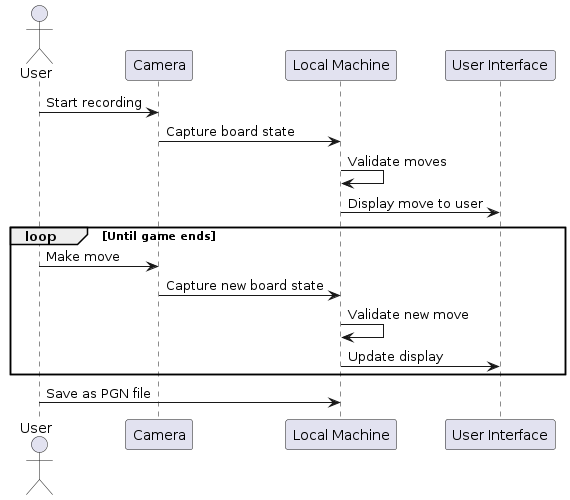
\includegraphics[width=0.75\linewidth]{figures/uml/sequence.png}
    \caption{Sequence Diagram}
    \label{fig:sequence}
\end{figure}

\begin{figure}[h!]
    \centering
    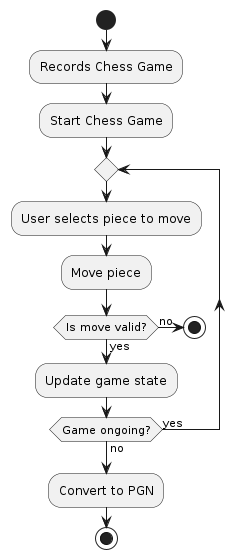
\includegraphics[height=0.75\linewidth]{figures/uml/activity.png}
    \caption{Activity Diagram}
    \label{fig:activity}
\end{figure}

\subsection{Design}

\subsubsection*{Wireframe}

\begin{figure}[h!]
    \centering
    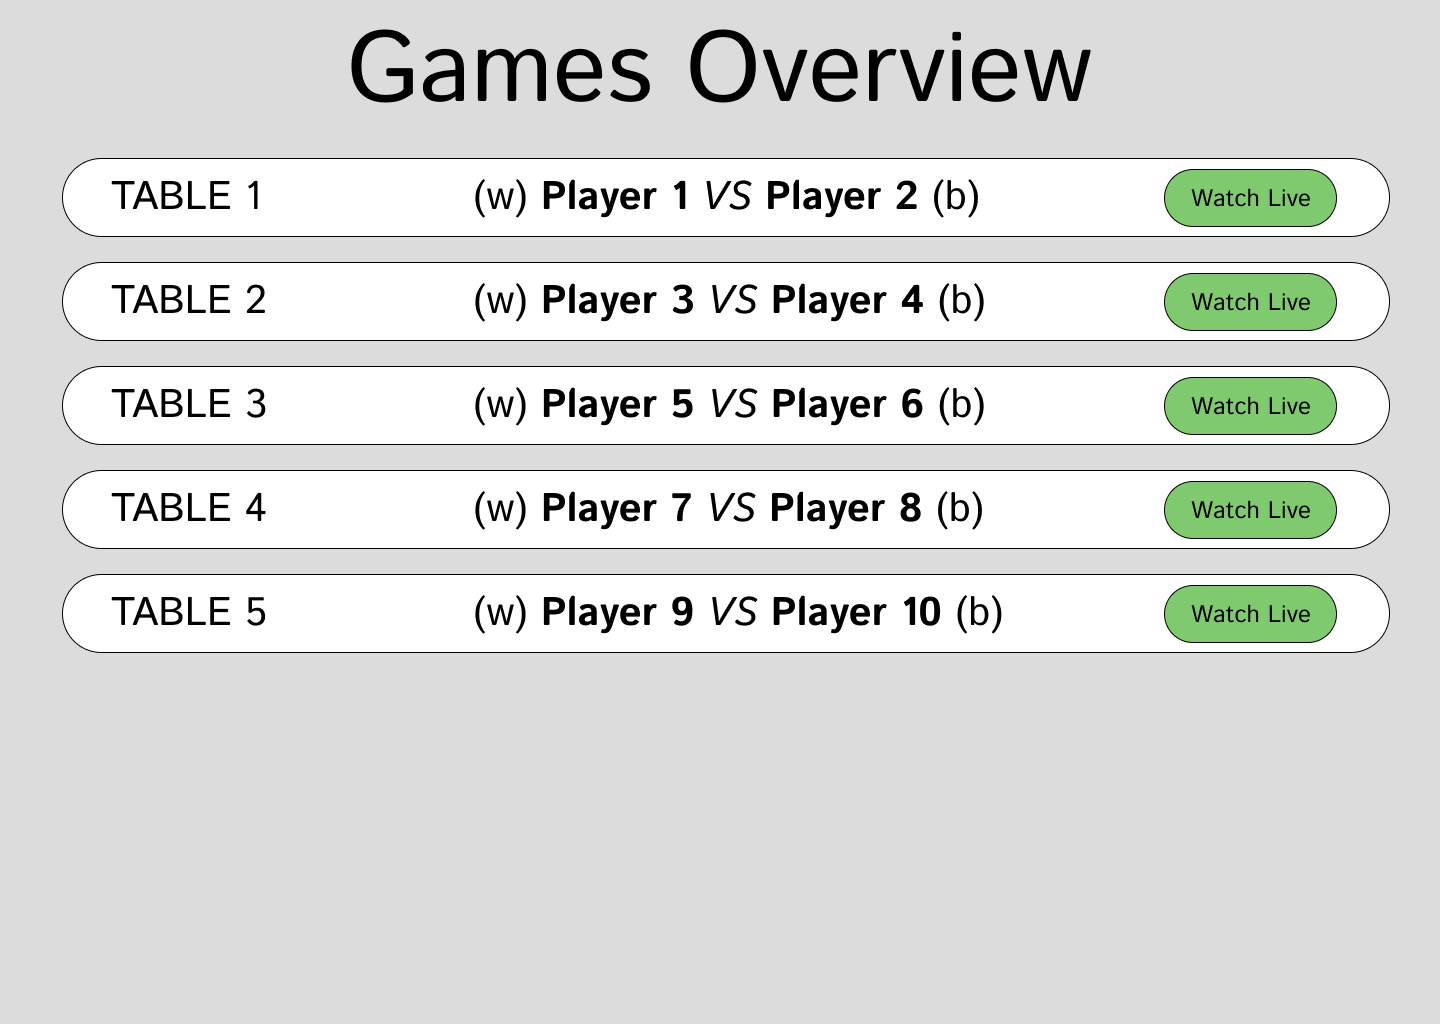
\includegraphics[width=0.75\linewidth]{figures/wireframe/overview.png}
    \caption{Wireframe of the Games Overview}
    \label{fig:app-overview}
\end{figure}


\begin{figure}[h!]
    \centering
    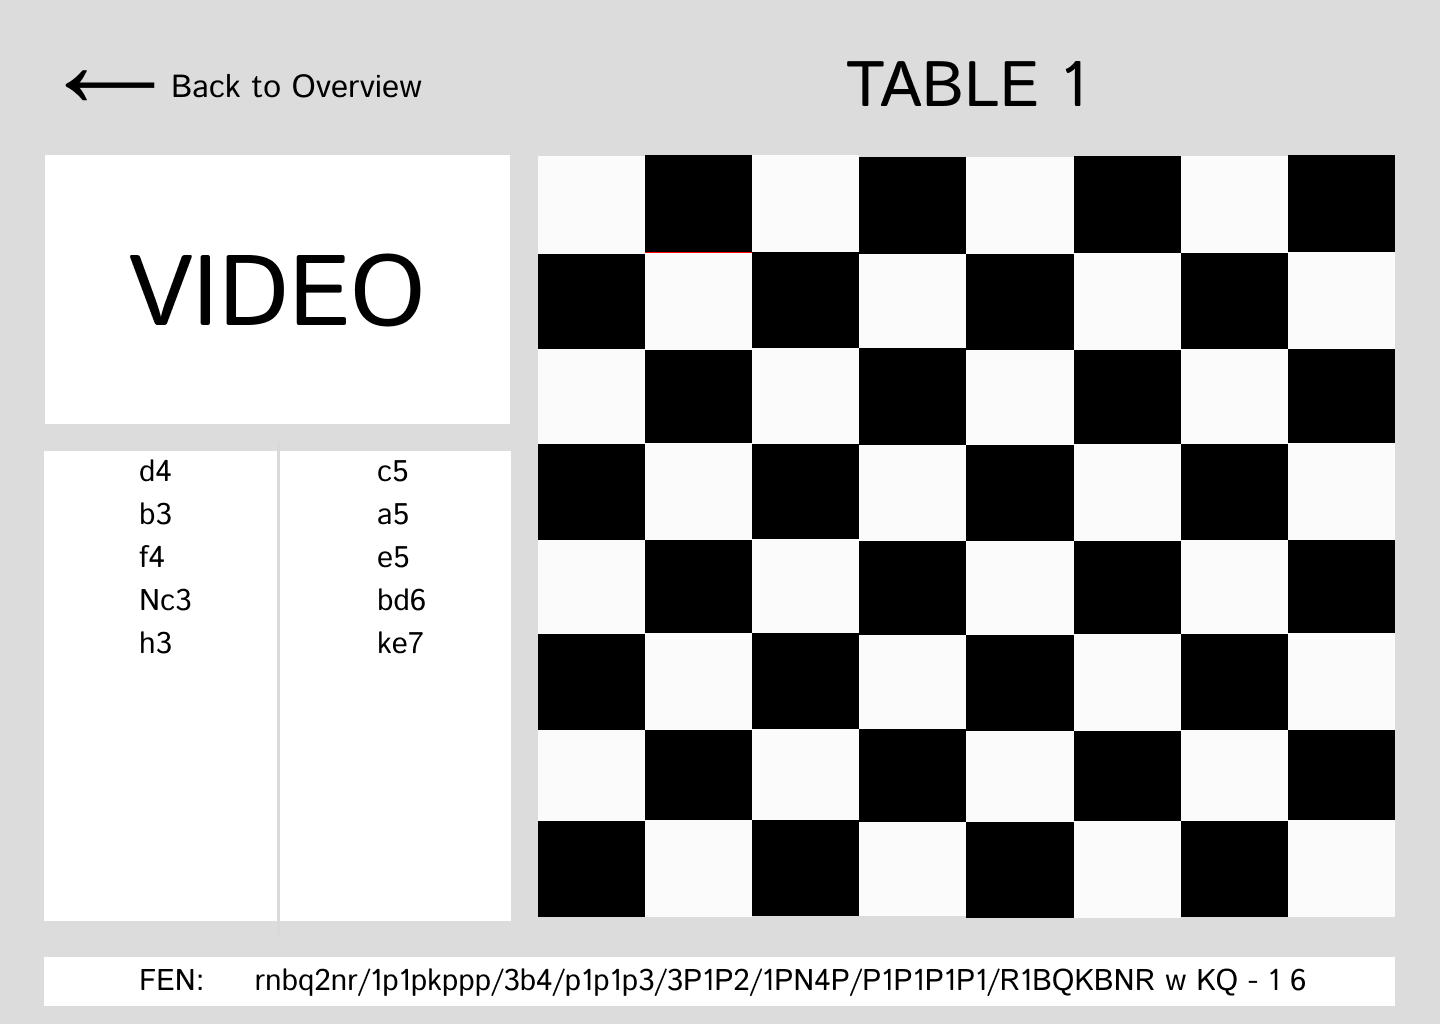
\includegraphics[width=0.75\linewidth]{figures/wireframe/table-view.png}
    \caption{Wireframe of the Table View of a Game on Table 1}
    \label{fig:app-table-view}
\end{figure}


% \subsection{User-Centered Design}



\section{Tools and Platforms}



\subsection{Development}



% \subsubsection*{Git}



% \subsubsection*{Postman}



% \subsubsection*{Visual Studio Code}



\subsection{Software Engineering}



% \subsubsection*{GitHub}



% \subsubsection*{Figma}



% \subsubsection*{OneDrive}



% \subsubsection*{Overleaf}



\section{Technology Stack}



\subsection{Backend}



% \subsubsection*{Python}



\subsection{Frontend}



% \subsubsection*{Vite}



% \subsubsection*{React}



% \subsubsection*{TypeScript}



% \subsubsection*{SWC}

